% Standalone source of the figure fig:staircase of the continuum-limit paper.
% Build: pdflatex fig_staircase.tex (or lualatex); the paper includes the PDF.
\documentclass[border=2pt]{standalone}
% Shared preamble of the continuum-limit paper's standalone figures.
\usepackage{amsmath,amssymb,bm}
\usepackage{tikz}
\usetikzlibrary{calc}
\newcommand{\bS}{\mathbf{S}}
\newcommand{\bG}{\mathbf{G}}
\newcommand{\bP}{\mathbf{P}}
\newcommand{\sinc}{\operatorname{sinc}}

\begin{document}
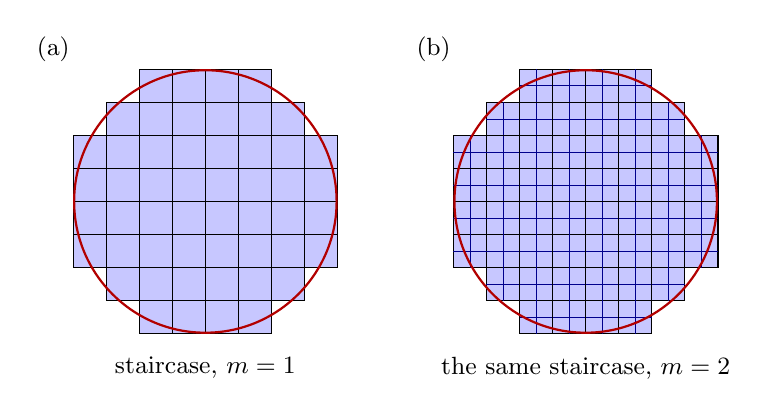
\begin{tikzpicture}[>=stealth, x=0.42cm, y=0.42cm, font=\small]
  % A cross-section through the n_sub = 8 voxelisation of a sphere of radius 4 (in units of the voxel
  % side), taken through a plane of voxel centres at height 1/2: a voxel belongs to the staircase when
  % its centre (x, y, 1/2) lies inside the sphere.
  % (a) the staircase at its own resolution, m = 1
  \begin{scope}
    \foreach \i in {0,...,7} \foreach \j in {0,...,7} {
      \pgfmathsetmacro{\cx}{\i - 3.5}
      \pgfmathsetmacro{\cy}{\j - 3.5}
      \pgfmathparse{(\cx*\cx + \cy*\cy + 0.25 < 16) ? 1 : 0}
      \ifnum\pgfmathresult=1 \draw[fill=blue!22] (\cx-0.5,\cy-0.5) rectangle (\cx+0.5,\cy+0.5); \fi
    }
    \draw[red!70!black, thick] (0,0) circle ({sqrt(16 - 0.25)});
    \node at (-4.6,4.6) {(a)};
    \node[below] at (0,-4.4) {staircase, $m=1$};
  \end{scope}
  % (b) the same staircase, every voxel split into 2 x 2 (x 2) sub-voxels: the shape does not change
  \begin{scope}[shift={(11.5,0)}]
    \foreach \i in {0,...,7} \foreach \j in {0,...,7} {
      \pgfmathsetmacro{\cx}{\i - 3.5}
      \pgfmathsetmacro{\cy}{\j - 3.5}
      \pgfmathparse{(\cx*\cx + \cy*\cy + 0.25 < 16) ? 1 : 0}
      \ifnum\pgfmathresult=1
        \draw[fill=blue!22] (\cx-0.5,\cy-0.5) rectangle (\cx+0.5,\cy+0.5);
        \draw[very thin, blue!55!black] (\cx,\cy-0.5) -- (\cx,\cy+0.5) (\cx-0.5,\cy) -- (\cx+0.5,\cy);
      \fi
    }
    \draw[red!70!black, thick] (0,0) circle ({sqrt(16 - 0.25)});
    \node at (-4.6,4.6) {(b)};
    \node[below] at (0,-4.4) {the same staircase, $m=2$};
  \end{scope}
\end{tikzpicture}
\end{document}
